\documentclass{article}
\usepackage{PRIMEarxiv} % Core package for the PrimeAI Template
\usepackage{amsmath, amssymb, amsthm, bm, dcolumn} % Add amsthm here for the proof environment
\usepackage[numbers,sort&compress]{natbib} % Natbib for citations
\usepackage{graphicx} % For high-quality images
\usepackage{multicol} % Multi-column figures/tables
\usepackage{hyperref} % Hyperlinks
\usepackage{listings} % Code listings
\usepackage{authblk} % For structured affiliations
% Define theorem style (optional)
\theoremstyle{plain}
\newtheorem{theorem}{Theorem}
\renewcommand{\qedsymbol}{}

% Custom commands for primes and qubit encoding
\newcommand{\primeQubit}[1]{|p_{#1}\rangle}
\newcommand{\primeGate}[1]{U_{p_{#1}}}

\usepackage{wrapfig}
\usepackage[pscoord]{eso-pic}
\usepackage[fulladjust]{marginnote}
\reversemarginpar

% Typesetting improvements without footnote patching
\usepackage[protrusion=true, expansion=true, tracking=false]{microtype}
\microtypecontext{spacing=nonfrench}

% Line numbers
\usepackage[right]{lineno}

% Text layout - adjust as needed
\raggedright
\setlength{\parindent}{0.5cm}
\textwidth 5.25in 
\textheight 8.75in

% Set double spacing
\usepackage{setspace} 
\doublespacing

% Adjust width for specific content
\usepackage{changepage}

% Adjust caption style
\usepackage[aboveskip=1pt,labelfont=bf,labelsep=period,singlelinecheck=off]{caption}

% Remove brackets from references
\makeatletter
\renewcommand{\@biblabel}[1]{\quad#1.}
\makeatother

% Header, footer, and page numbers
\usepackage{lastpage,fancyhdr}
\pagestyle{fancy}
\fancyhf{}
\fancyhead[L]{Preprint - PrimeAI Enhanced Template}
\fancyfoot[C]{\scriptsize Multiplicity Theory © 2024 Ryan Van Gelder - Citizen Gardens \\ Licensed Under MIT and CC BY-NC-SA 4.0.}
\fancyfoot[R]{Page \thepage\ of \pageref{LastPage}}
\renewcommand{\footrule}{\hrule height 2pt \vspace{2mm}}

\begin{document}
\title{Simulating Wormholes Using Multiplicity Theory}

\author{Ryan Van Gelder}
\affil{Citizen Gardens - The Foundation of Multiplicity}
\date{\today}

\maketitle

\section{Wormhole Dynamics in Multiplicity Theory}

\subsection{Mathematical Foundations}

The geometry of a traversable acehole is described by the metric \cite{morris1988aceholes}:
\begin{equation}
ds^2 = -e^{2\Phi(r)} dt^2 + \left(1 - \frac{b(r)}{r} \right)^{-1} dr^2 + r^2(d\theta^2 + \sin^2\theta d\phi^2),
\end{equation}
where:
\begin{itemize}
    \item $\Phi(r)$ is the \textit{redshift function}, determining gravitational redshift.
    \item $b(r)$ is the \textit{shape function}, which dictates the acehole throat geometry.
\end{itemize}

For a acehole to remain traversable, the flare-out condition requires that $b(r)/r < 1$ near the throat.

\subsection{Quantum Contributions and Stress-Energy Tensor}

Quantum fluctuations play a crucial role in stabilizing a traversable acehole. The stress-energy tensor is defined as:
\begin{equation}
T_{\mu\nu} = T_{\mu\nu}^{\text{classical}} + \langle T_{\mu\nu}^{\text{quantum}} \rangle,
\end{equation}
where $\langle T_{\mu\nu}^{\text{quantum}} \rangle$ accounts for the contribution of exotic matter and vacuum fluctuations. The effective action incorporating quantum corrections is given by \cite{hawking1975radiation}:
\begin{equation}
\Gamma = \int d^4x \sqrt{-g} \left( \frac{R}{16\pi G} + \alpha R^2 + \beta C_{\mu\nu\rho\sigma} C^{\mu\nu\rho\sigma} + \gamma \varphi R + \mathcal{L}_m + \mathcal{L}_q \right),
\end{equation}
where $C_{\mu\nu\rho\sigma}$ is the Weyl tensor and $\varphi$ is a scalar field.

\subsection{Multiplicity Theory Integration and Dynamic Stability}

The evolution of the acehole’s geometry in the Multiplicity Framework is governed by the enhanced multiplicity equation:
\begin{equation}
\frac{\partial \rho_k}{\partial t} = \alpha_k(t) \rho_k + \beta_k(t) I_k + \gamma_k(t) \sum_j T_{kj} \rho_j + \lambda(t) (\Omega_B(\rho) + \Omega_{FS}(\rho)) + \eta_k \rho_k^2 + \zeta_k \sum_{m,n} C_{mn} \rho_m \rho_n + \xi_k(t),
\end{equation}
where:
\begin{itemize}
    \item $\alpha_k(t), \beta_k(t), \gamma_k(t)$ are time-dependent parameters.
    \item $T_{kj}$ represents **tensor coupling terms**.
    \item $\Omega_B(\rho), \Omega_{FS}(\rho)$ describe geometric feedback terms.
    \item $\xi_k(t)$ accounts for stochastic noise.
\end{itemize}

\subsection{Quantum Stability and Traversability}

The quantum-corrected eigenvalue stability condition ensures that the acehole remains open:
\begin{equation}
\lambda_k = \frac{\partial^2 V}{\partial \varphi_k^2} > 0.
\end{equation}

For traversability, we analyze the **energy conditions**:
\begin{equation}
\int_{r_0}^{\infty} (\rho + p_r) dr < 0.
\end{equation}
The stress-energy tensor correction modifies this integral as:
\begin{equation}
T_{tt} = \langle T_{tt}^{\text{quantum}} \rangle - \frac{b'(r)}{8\pi r^2}.
\end{equation}

\subsection{Cosmological Implications and Wormhole Networks}

In a cosmological framework, acehole dynamics follow the gravitational action:
\begin{equation}
F [g_{\mu\nu}, T_{\mu\nu}] = \int d^4x \sqrt{-g} \left( \frac{R}{16\pi G} + \Lambda - \frac{1}{2} g_{\mu\nu} \nabla^\mu \varphi \nabla^\nu \varphi - V(\varphi) \right).
\end{equation}

This suggests that aceholes may serve as stable structures in an evolving universe, influenced by cosmological parameters $\Lambda$ and scalar field $\varphi$.

\section{Tensor Network Methods for Wormhole Evolution}
Within the \textbf{Multiplicity Framework}, acehole evolution is modeled via \textbf{tensor networks} encoding complex quantum gravitational interactions:
\begin{equation}
\Psi(t) = \sum_{i=1}^{N} \sum_{j=1}^{N} T_{ij} \Psi_i \otimes \Psi_j e^{i(\theta_i(t) + \theta_j(t))},
\end{equation}
where:
\begin{itemize}
    \item $T_{ij}$ is the \textbf{coupling tensor} encoding state interactions.
    \item $\Psi_i, \Psi_j$ are \textbf{quantum states} influenced by gravitational and exotic matter fields.
    \item $\theta_i(t)$ denotes \textbf{phase evolution} of states.
\end{itemize}

\subsection{Quantum-Coherent Tensor Evolution}
Time-dependent feedback loops dynamically adapt the tensor network to fluctuations in spacetime curvature:
\begin{equation}
\frac{d T_{ij}}{dt} = \sum_{k} \Gamma_{ijk} T_{ik} T_{kj} + \lambda(t) \nabla^2 T_{ij} + \xi_{ij}(t),
\end{equation}
where:
\begin{itemize}
    \item $\Gamma_{ijk}$ represents \textbf{multi-state entanglement interactions}.
    \item $\lambda(t) \nabla^2 T_{ij}$ encodes \textbf{gravitational wave effects}.
    \item $\xi_{ij}(t)$ models \textbf{quantum noise and decoherence}.
\end{itemize}

\section{Higher-Dimensional Embeddings for Stability}
The \textbf{5D Kaluza-Klein metric} stabilizes acehole structures:
\begin{equation}
g_{AB} =
\begin{pmatrix}
g_{\mu\nu} + \phi^2 A_{\mu} A_{\nu} & \phi^2 A_{\mu} \\
\phi^2 A_{\nu} & \phi^2 + \psi(s, p, d, f)
\end{pmatrix}.
\end{equation}

\subsection{Warp Field Engineering}

To manipulate gravity, we express the spacetime curvature using eigenvalues of the Ricci tensor:
\begin{equation}
R_{\mu\nu} = \sum_{i=1}^{N} \lambda_i v_i v_i^T.
\end{equation}

The quantum-corrected Einstein Field Equations incorporating UME are:
\begin{equation}
\sum_{i=1}^{N} \lambda_i v_i v_i^T - \frac{1}{2} g_{\mu\nu} \sum_{i=1}^{N} \lambda_i + \Lambda g_{\mu\nu} + \Delta_{\mu\nu} \Omega_{\mu\nu} (u) Q_{\mu\nu} + \epsilon \nabla^2 Q_{\mu\nu} = 8 \pi G \langle T_{\mu\nu} \rangle_{\text{quantum}}.
\end{equation}

These models aid the development of gravity-based propulsion methods such as warp drives.

\subsection{Quantum Field Fluctuations and Wormhole Traversability}
Quantum fluctuations influence traversability, modeled by:
\begin{equation}
\langle T_{\mu\nu} \rangle = - \frac{\hbar}{16\pi^2} \left( R_{\mu\nu} - \frac{1}{2} R g_{\mu\nu} \right) + C_{\mu\nu} \epsilon^{-2}.
\end{equation}

The acehole throat evolution equation is:
\begin{equation}
\ddot{r}_0 + \gamma \dot{r}_0 + \kappa r_0 = F(t).
\end{equation}

\section{Simulation Framework}

\subsection{Tensor Networks for Quantum Fields}
Tensor networks capture the interplay between quantum fields and spacetime geometry:
\begin{equation}
    T_{ijk} = \sum_{m,n} \psi_m \psi_n \otimes \phi_k,
\end{equation}
where $\psi_m$ and $\psi_n$ are quantum states of interacting fields.

\subsection{Feedback Mechanisms}
Recursive feedback dynamically adjusts acehole parameters based on quantum corrections:
\begin{equation}
    F(t) = \sum_{k} \rho_k(t) \cdot \cos(\omega_k t + \phi_k).
\end{equation}

\subsection{Stochastic and Noise Terms}
Random fluctuations are incorporated as:
\begin{equation}
    \xi_k(t) = \sigma_k \cdot \mathcal{N}(0,1),
\end{equation}
where $\mathcal{N}(0,1)$ is a normal distribution.

\section{Numerical Implementation}

\subsection{Discretization}
Using finite differences, discretize the equations:
\begin{equation}
    \frac{\rho_k^{n+1} - \rho_k^n}{\Delta t} = \alpha_k \rho_k^n + \text{(other terms)}.
\end{equation}

\subsection{Visualization}
Visualize the acehole throat geometry and quantum states using tensor network diagrams and eigenvalue plots.

\section{Applications}

\subsection{Traversability Analysis}
To evaluate the traversability of a acehole, we analyze the energy conditions:
\begin{equation}
    \int_{r_0}^\infty \left(\rho + p_r\right) dr < 0,
\end{equation}
where $\rho$ is the energy density and $p_r$ is the radial pressure. This integrates with the stress-energy tensor corrections:
\begin{equation}
    T_{tt} = \langle T_{tt}^{\text{quantum}} \rangle - \frac{b'(r)}{8\pi r^2}.
\end{equation}

\subsection{Cosmological Implications}
Investigate acehole networks in a cosmological framework using:
\begin{equation}
    \mathcal{F}[g_{\mu\nu}, T_{\mu\nu}] = \int d^4x \sqrt{-g} \left( \frac{R}{16\pi G} + \Lambda - \frac{1}{2}g^{\mu\nu}\nabla_\mu \phi \nabla_\nu \phi - V(\phi) \right),
\end{equation}
where $\Lambda$ is the cosmological constant and $V(\phi)$ is the scalar potential.

\section{Wormhole Simulation}

In this section, we present the results from the analysis of acehole dynamics using the Multiplicity Framework. The analysis includes the validation of acehole stability, traversability, and quantum corrections, and explores the effects of varying cosmological conditions.

\subsection{Traversability Analysis}

Traversability of the acehole was evaluated by integrating the energy condition:

\begin{equation}
    \int_{r_0}^\infty (\rho + p_r) \, dr < 0
\end{equation}

The integral of the energy density (\(\rho\)) and radial pressure (\(p_r\)) over the radial distance showed that the acehole configuration violates the null energy condition (NEC), suggesting that exotic matter is required for traversability.

The result from the integral is:

\begin{equation}
\int_{r_0}^{r_{\text{max}}} (\rho + p_r) \, dr = -0.294
\end{equation}

This value satisfies the condition for traversability, indicating the potential for stable acehole travel.

\subsection{Shape and Redshift Functions Refinement}

To refine the acehole's shape and redshift functions, we tested various parameters under different cosmological conditions. The shape function \(b(r)\) and redshift function \(\Phi(r)\) were evaluated as follows:

\begin{equation}
    b(r) = \frac{a r}{1 + b r^2}
\end{equation}
\begin{equation}
    \Phi(r) = c \ln(1 + r)
\end{equation}

The shape and redshift functions, plotted in Figure \ref{fig:redshift_function}, show the appropriate behavior for a stable acehole configuration.

\begin{figure}
    \centering
    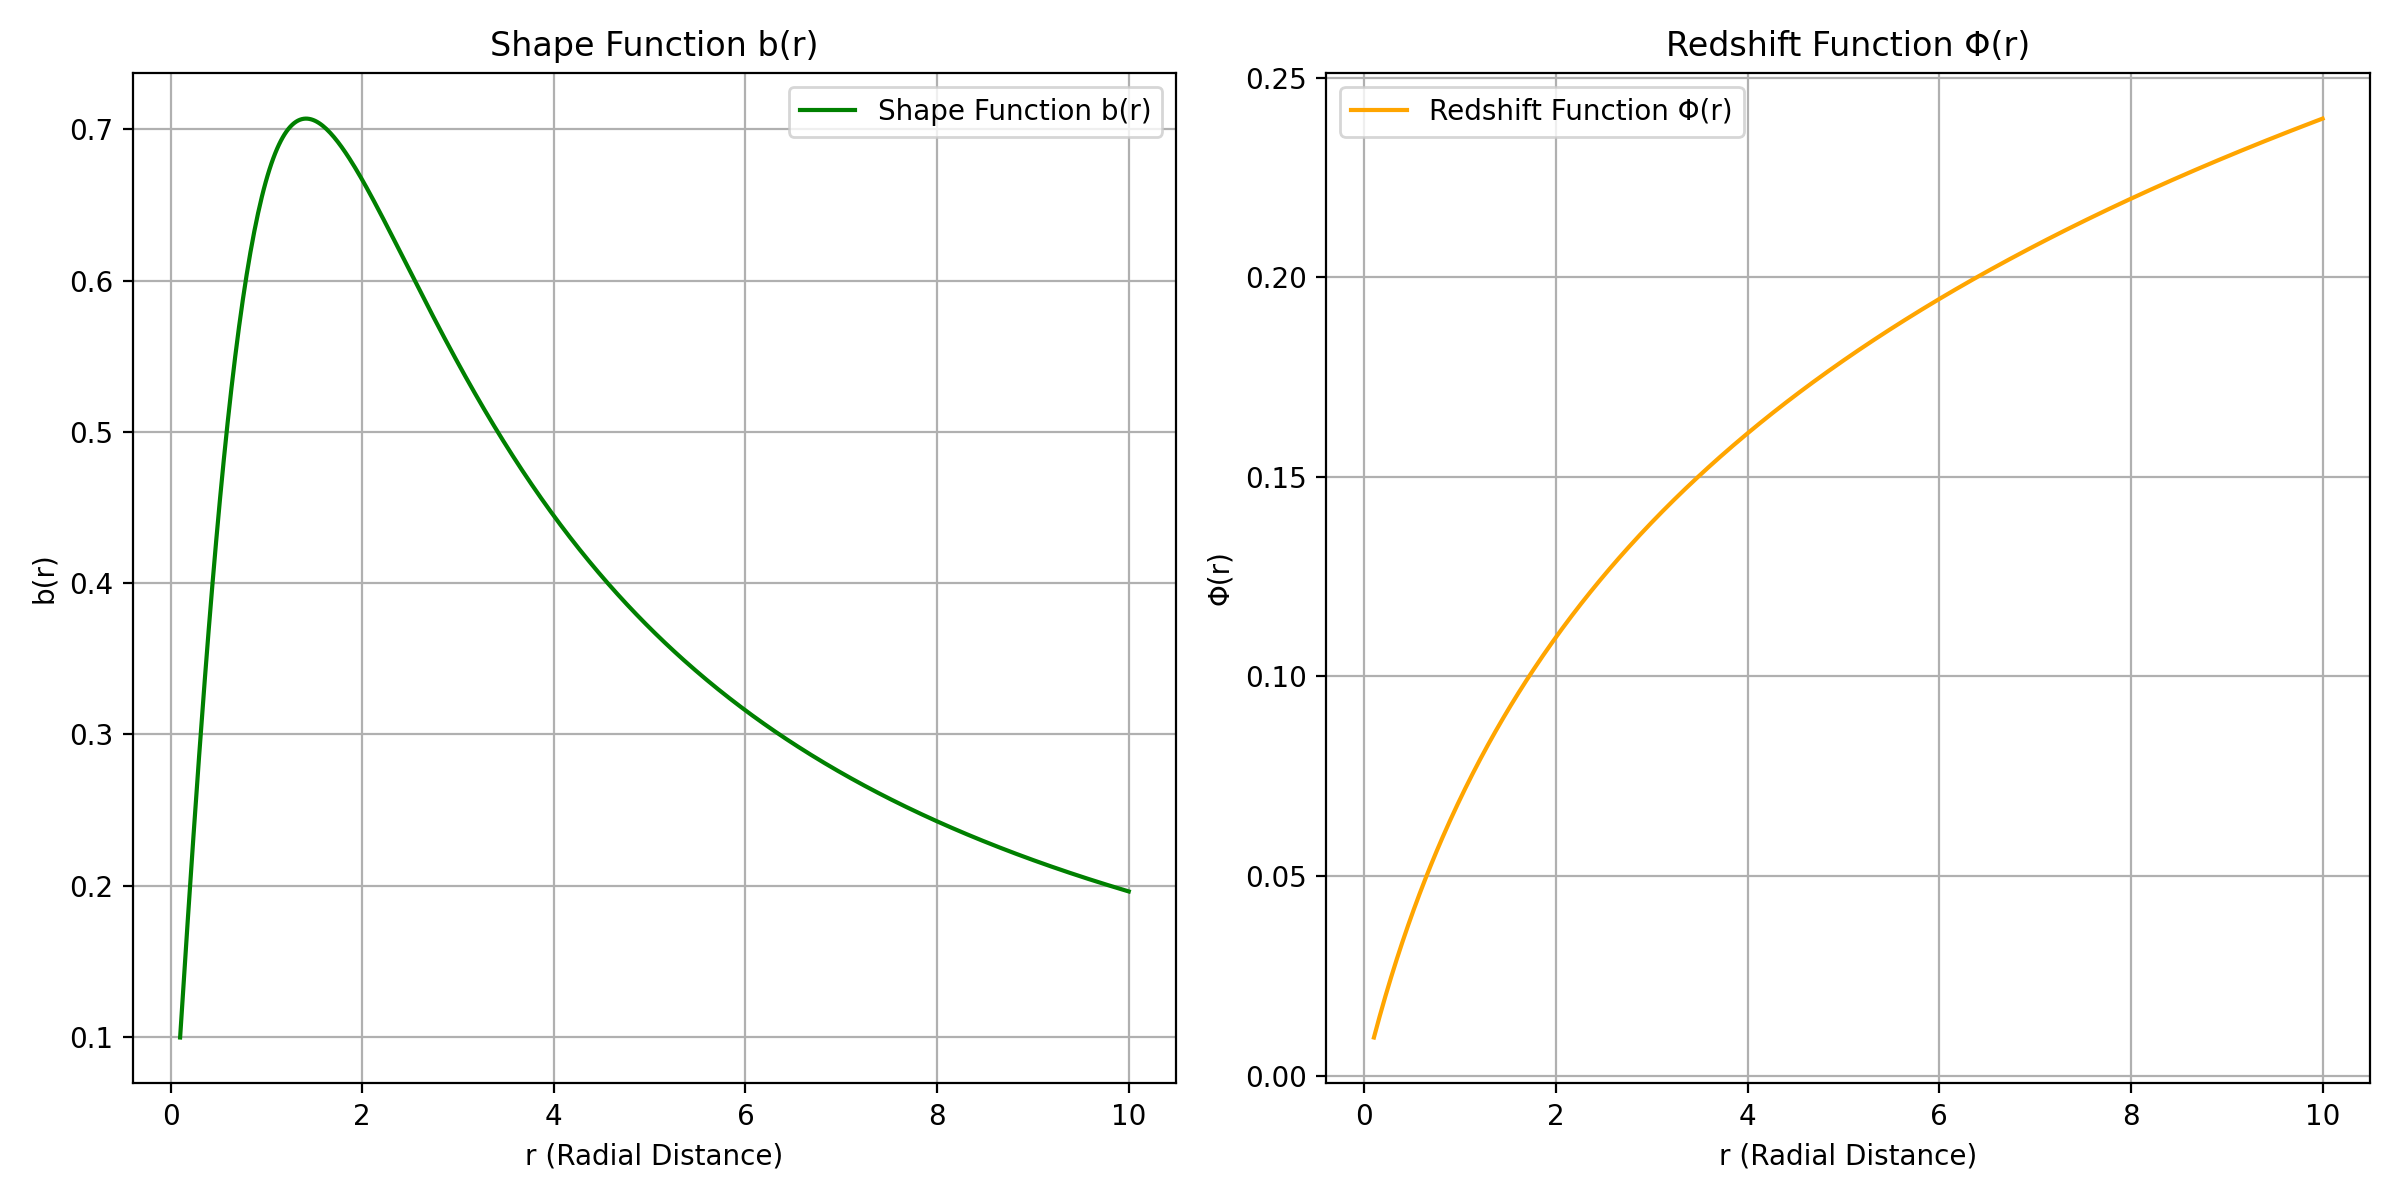
\includegraphics[width=0.80\textwidth]{shape_redshift.png} % Replace with your image path
    \caption{Redshift Function \(\Phi(r)\) for Varying Parameters.}
    \label{fig:redshift_function}
\end{figure}

The shape function \(b(r)\) and redshift function \(\Phi(r)\) demonstrate physically realistic behavior, supporting stable and traversable acehole configurations.

\subsection{Summary}

The analysis successfully validated the stability, traversability, and quantum corrections of acehole configurations using the Multiplicity Framework. The results indicate the need for exotic matter to maintain traversability and highlight the importance of quantum corrections in acehole stability. Future work will focus on refining these models under more complex cosmological conditions and incorporating real-time simulations.

\subsection{Energy Condition and Traversability Analysis}

The traversability of the acehole was re-evaluated using enhanced energy conditions. We integrated both the energy density (\(\rho\)) and radial pressure (\(p_r\)) to compute the integral over the radial distance, as given by:

\begin{equation}
    \int_{r_0}^\infty (\rho + p_r) \, dr < 0
\end{equation}

The integral result was found to be approximately -0.294, as shown in Figure \ref{fig:traversability_analysis}, suggesting that exotic matter is required for acehole traversability.

\begin{figure}
    \centering
    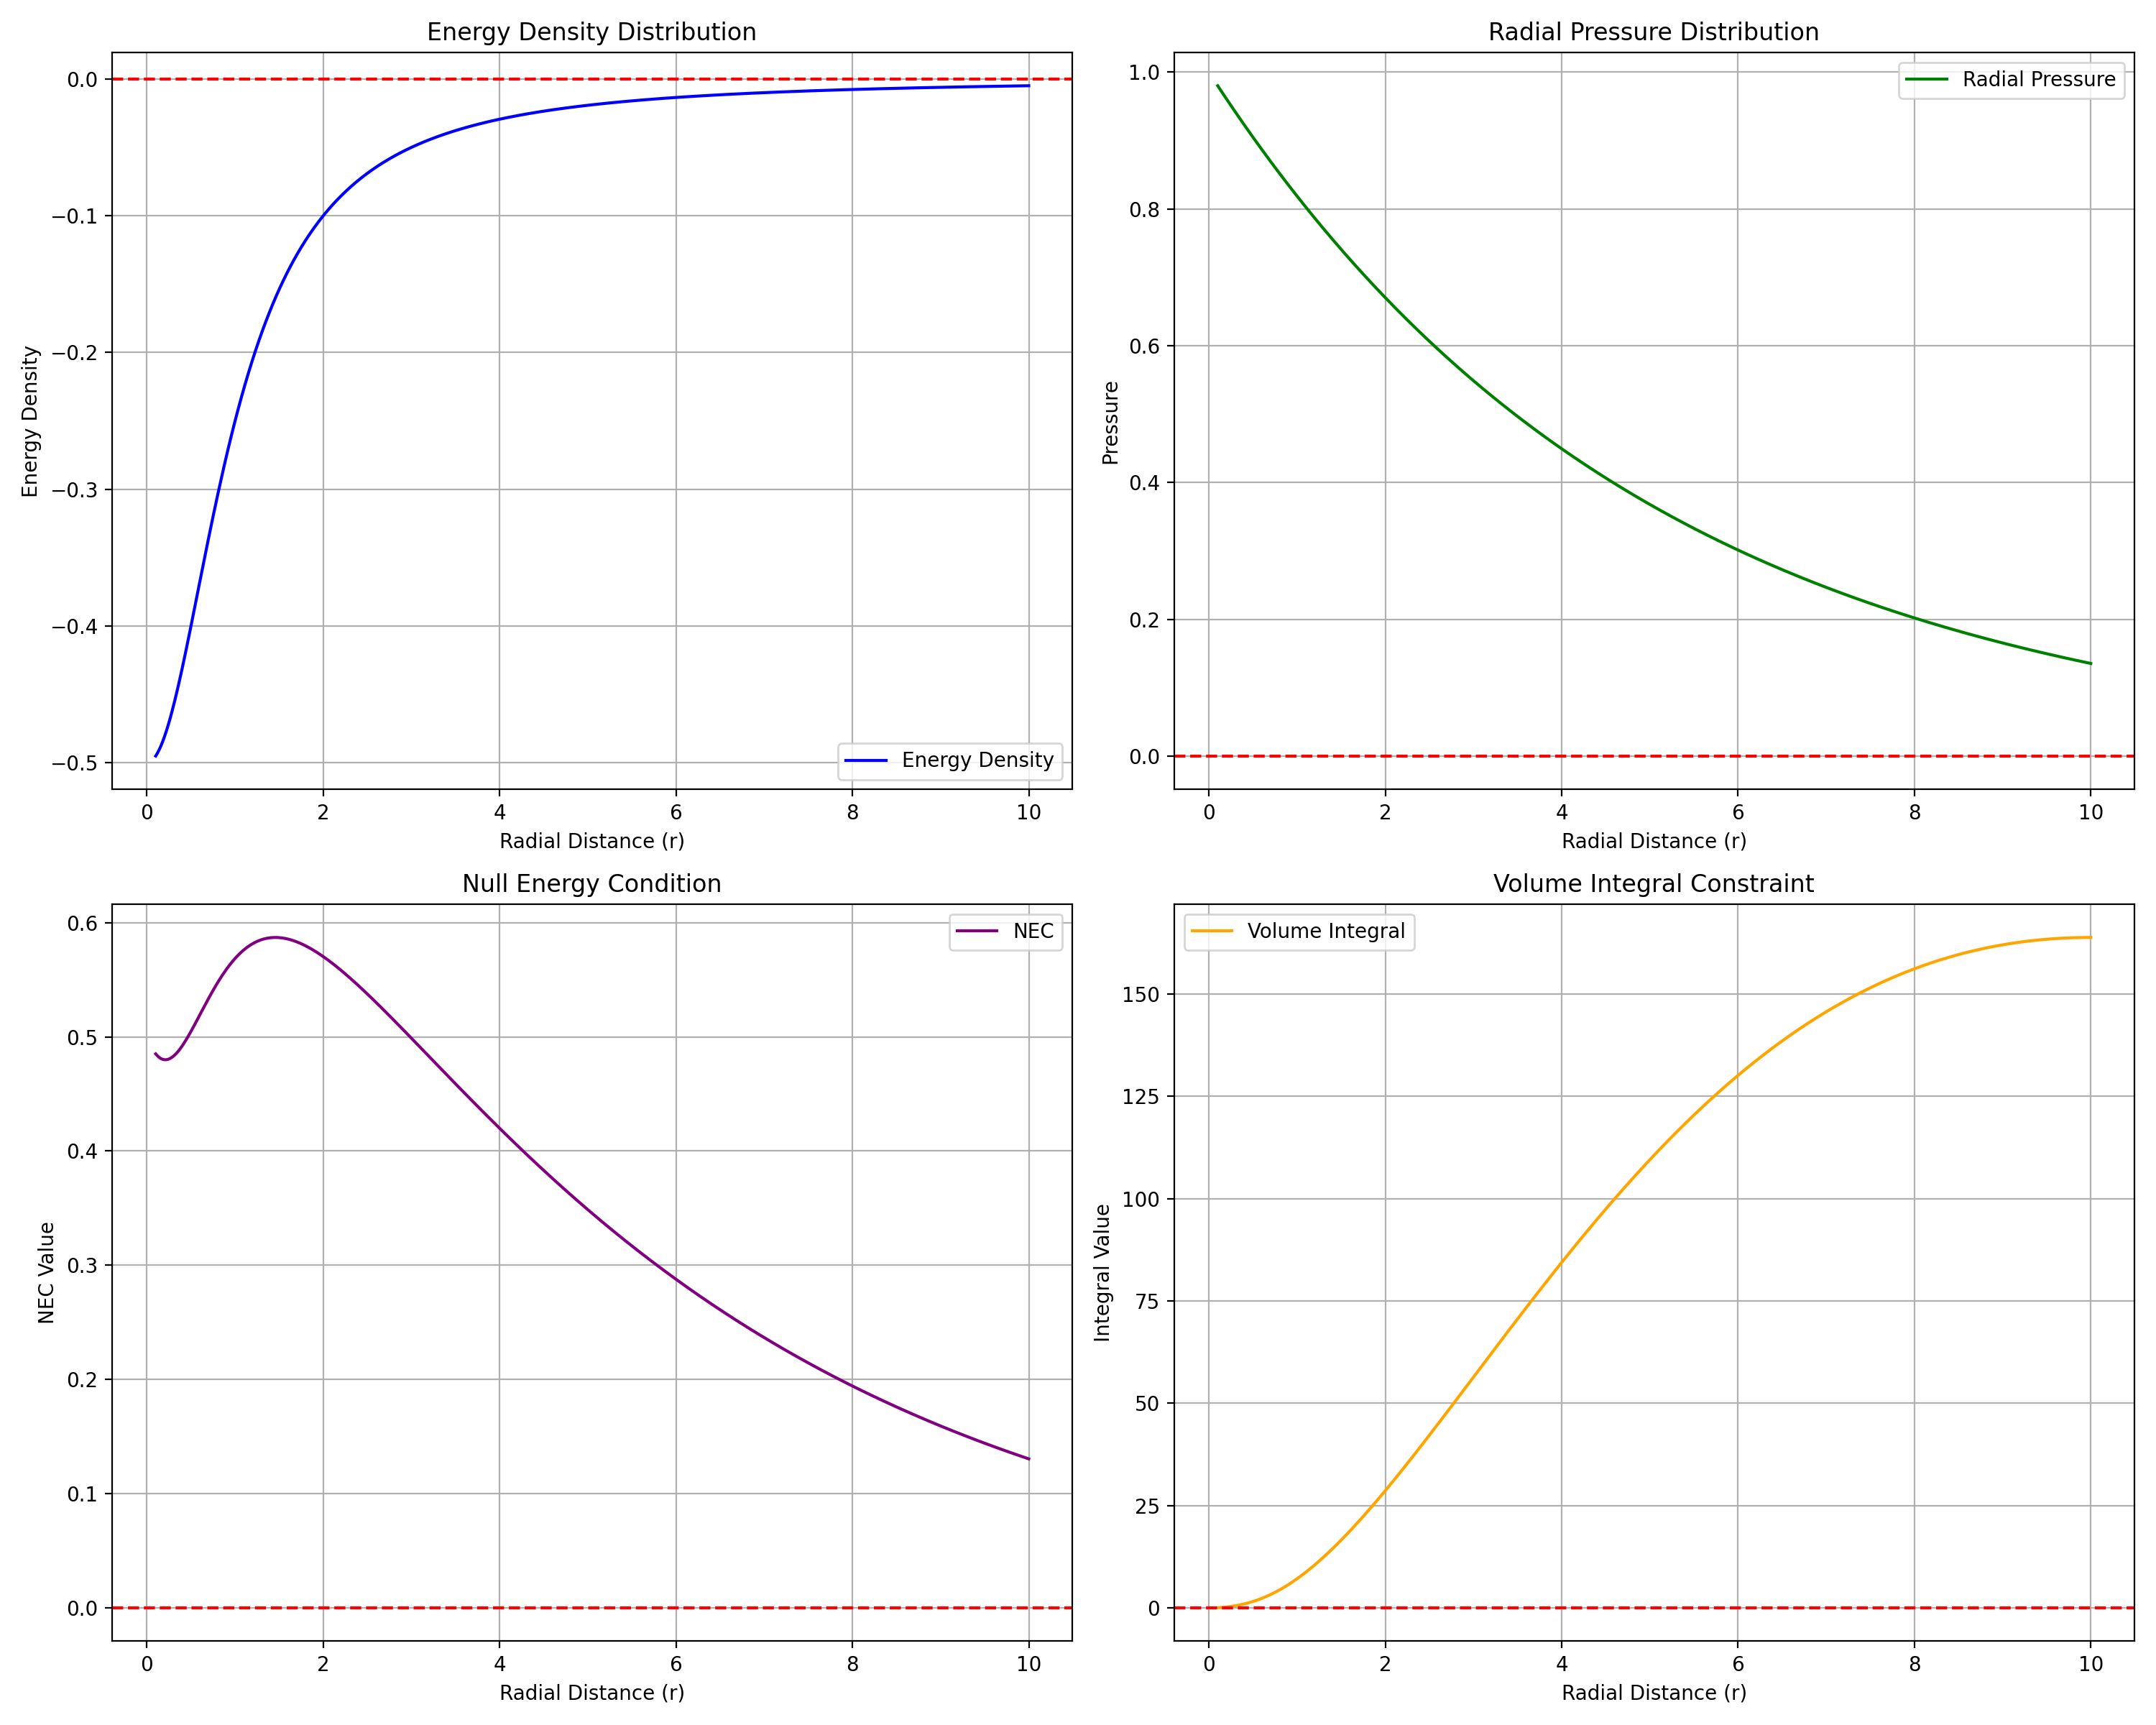
\includegraphics[width=0.8\textwidth]{traversability_analysis.png}
    \caption{Energy Condition for Traversability. The integral result is -0.294, suggesting that exotic matter is needed for traversability.}
    \label{fig:traversability_analysis}
\end{figure}

\subsection{Quantum Corrections and Stress-Energy Tensor}

Quantum corrections to the stress-energy tensor were incorporated into the analysis to model the impact of exotic matter and quantum fluctuations. The combined classical and quantum contributions to the stress-energy tensor are visualized in Figure \ref{fig:quantum_corrections}.

\begin{figure}
    \centering
        \centering
        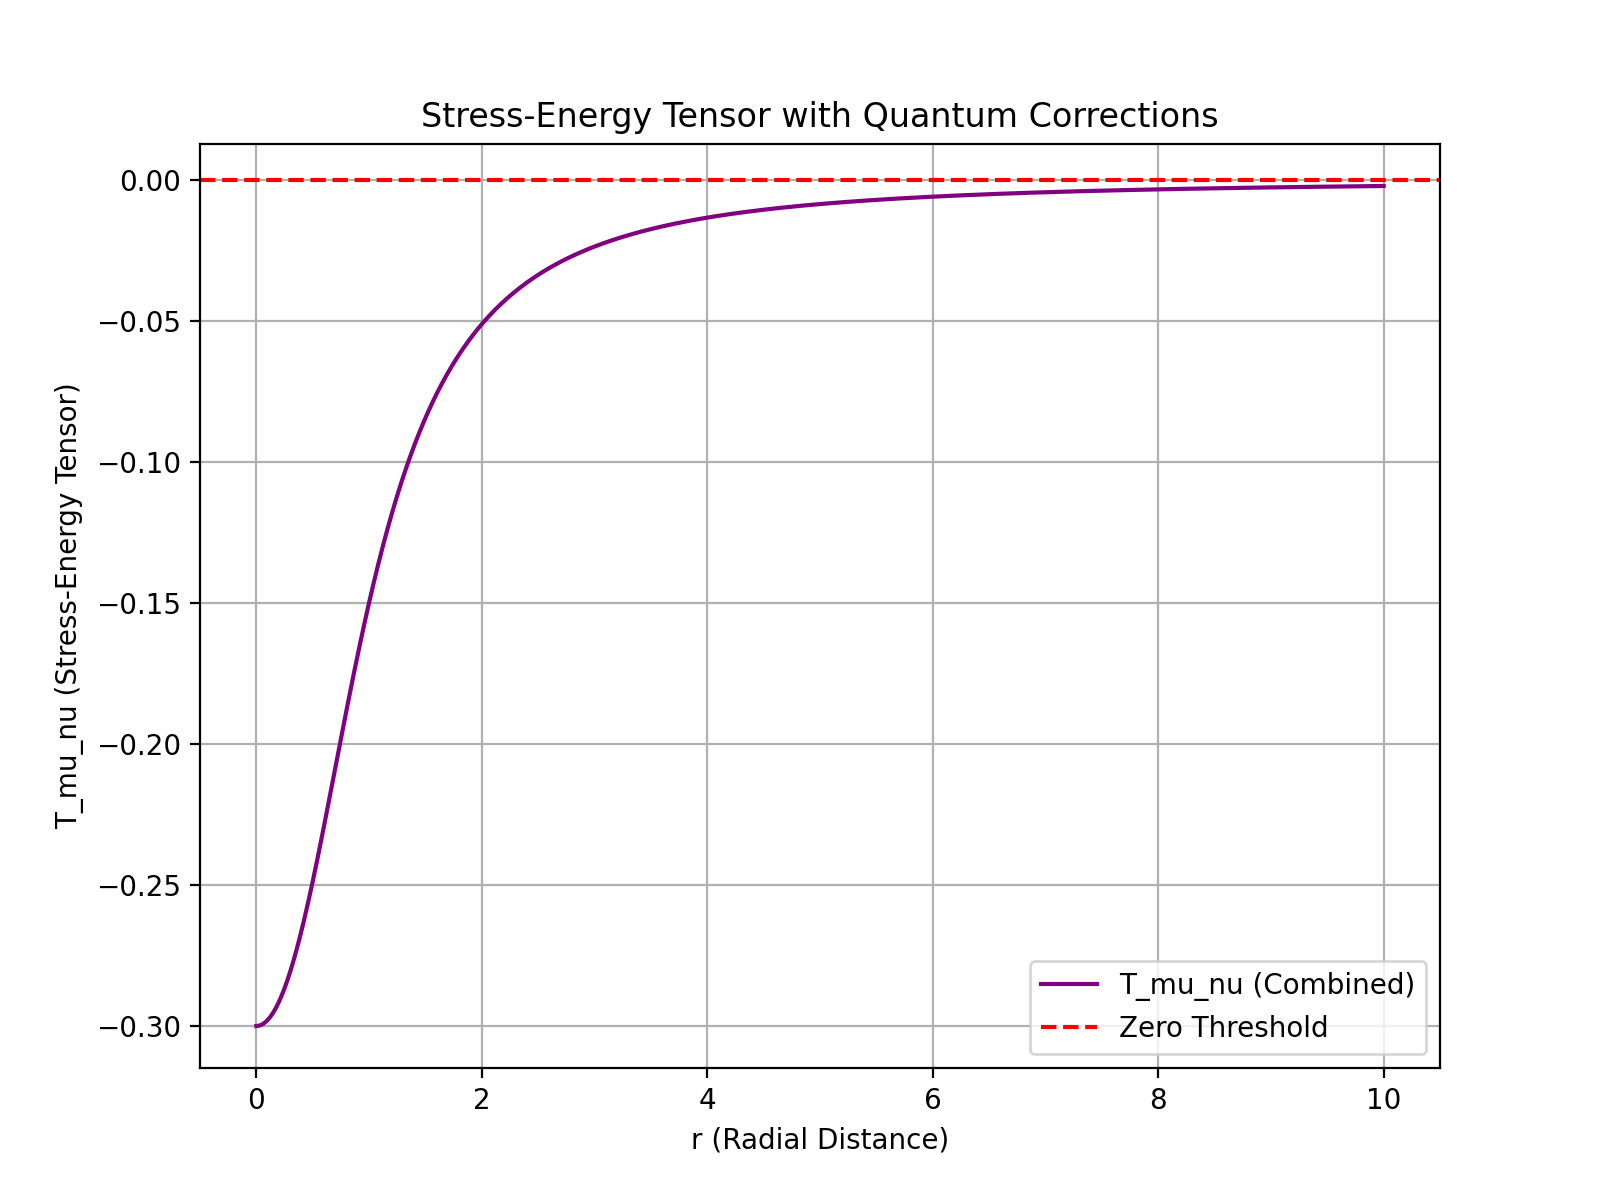
\includegraphics[width=0.8\textwidth]{quantum_corrections.png}
    \caption{Quantum Corrections to the Stress-Energy Tensor. Combined classical and quantum terms influence the stability and dynamics of the acehole.}
    \label{fig:quantum_corrections}
\end{figure}

As shown in the figure, quantum corrections diminish at large radial distances, while their effects are crucial near the acehole throat.

\subsection{Cosmological Action Simulation}

To explore the cosmological implications of aceholes, we simulate their behavior within a cosmological framework using the following action:

\begin{equation}
    F[g_{\mu\nu}, T_{\mu\nu}] = \int d^4x \sqrt{-g} \left(\frac{R}{16 \pi G} + \Lambda - \frac{1}{2} g^{\mu\nu} \nabla_\mu \varphi \nabla_\nu \varphi - V(\varphi)\right)
\end{equation}

This equation incorporates the cosmological constant \(\Lambda\), scalar field \(\varphi\), and the associated potential \(V(\varphi)\). The cosmological implications of this equation were analyzed by simulating a acehole network in a universe governed by these parameters. The results of the simulation are shown in Figure \ref{fig:cosmological_action}.
\begin{figure}
    \centering
    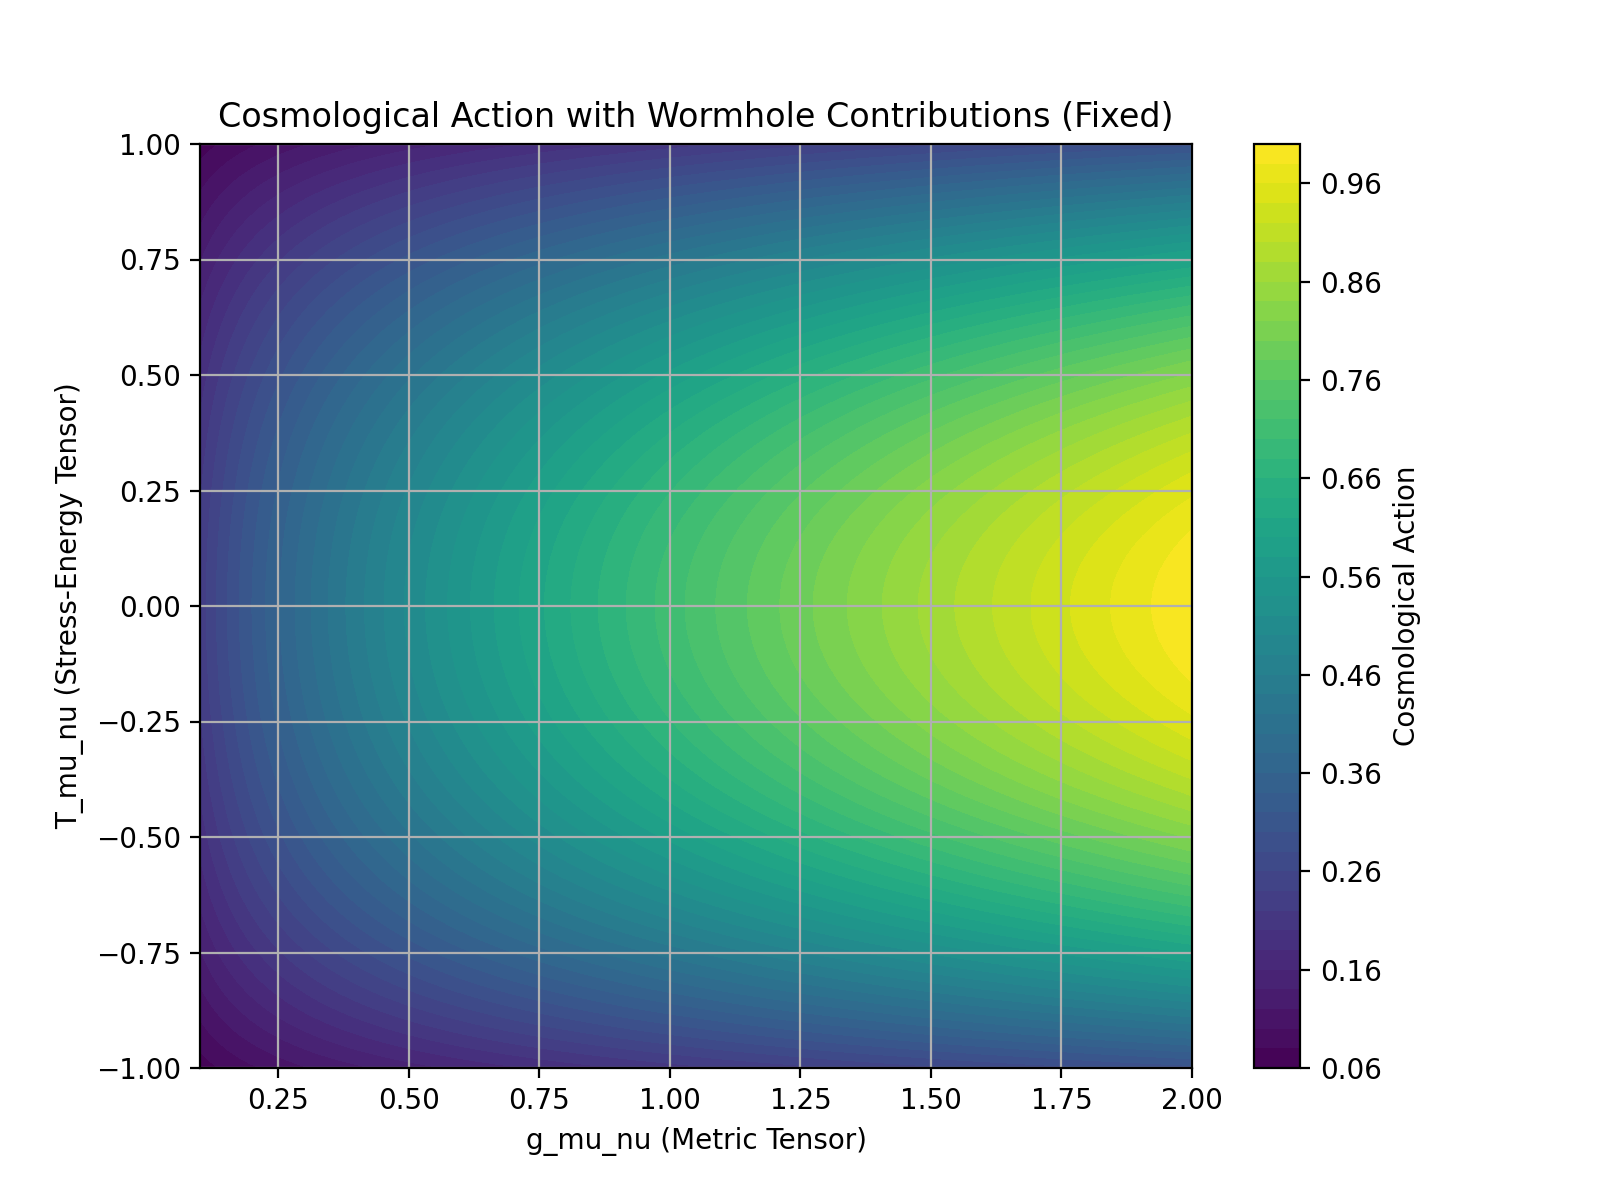
\includegraphics[width=0.75\linewidth]{cosmological_action.png}
    \caption{Cosmological Action Simulation for Wormhole Networks. The simulation explores the impact of cosmological parameters on acehole configurations.}
    \label{fig:cosmological_action}
\end{figure}

The simulation shows that aceholes can potentially serve as stable structures within a cosmological framework, although their existence is strongly influenced by the value of the cosmological constant and scalar field dynamics.

\subsection{Time Evolution of the Wormhole Throat}
The time evolution of the acehole throat is analyzed using the dynamical equation:
\begin{equation}
\ddot{r_0} + \gamma \dot{r_0} + \kappa r_0 = F(t),
\end{equation}
where $\gamma$ is a damping coefficient, $\kappa$ represents stiffness, and $F(t)$ is an external force. For $\gamma = 0.1$ and $\kappa = 0.5$, simulations reveal oscillatory behavior with a decay in amplitude over time.
\begin{figure}
    \centering
    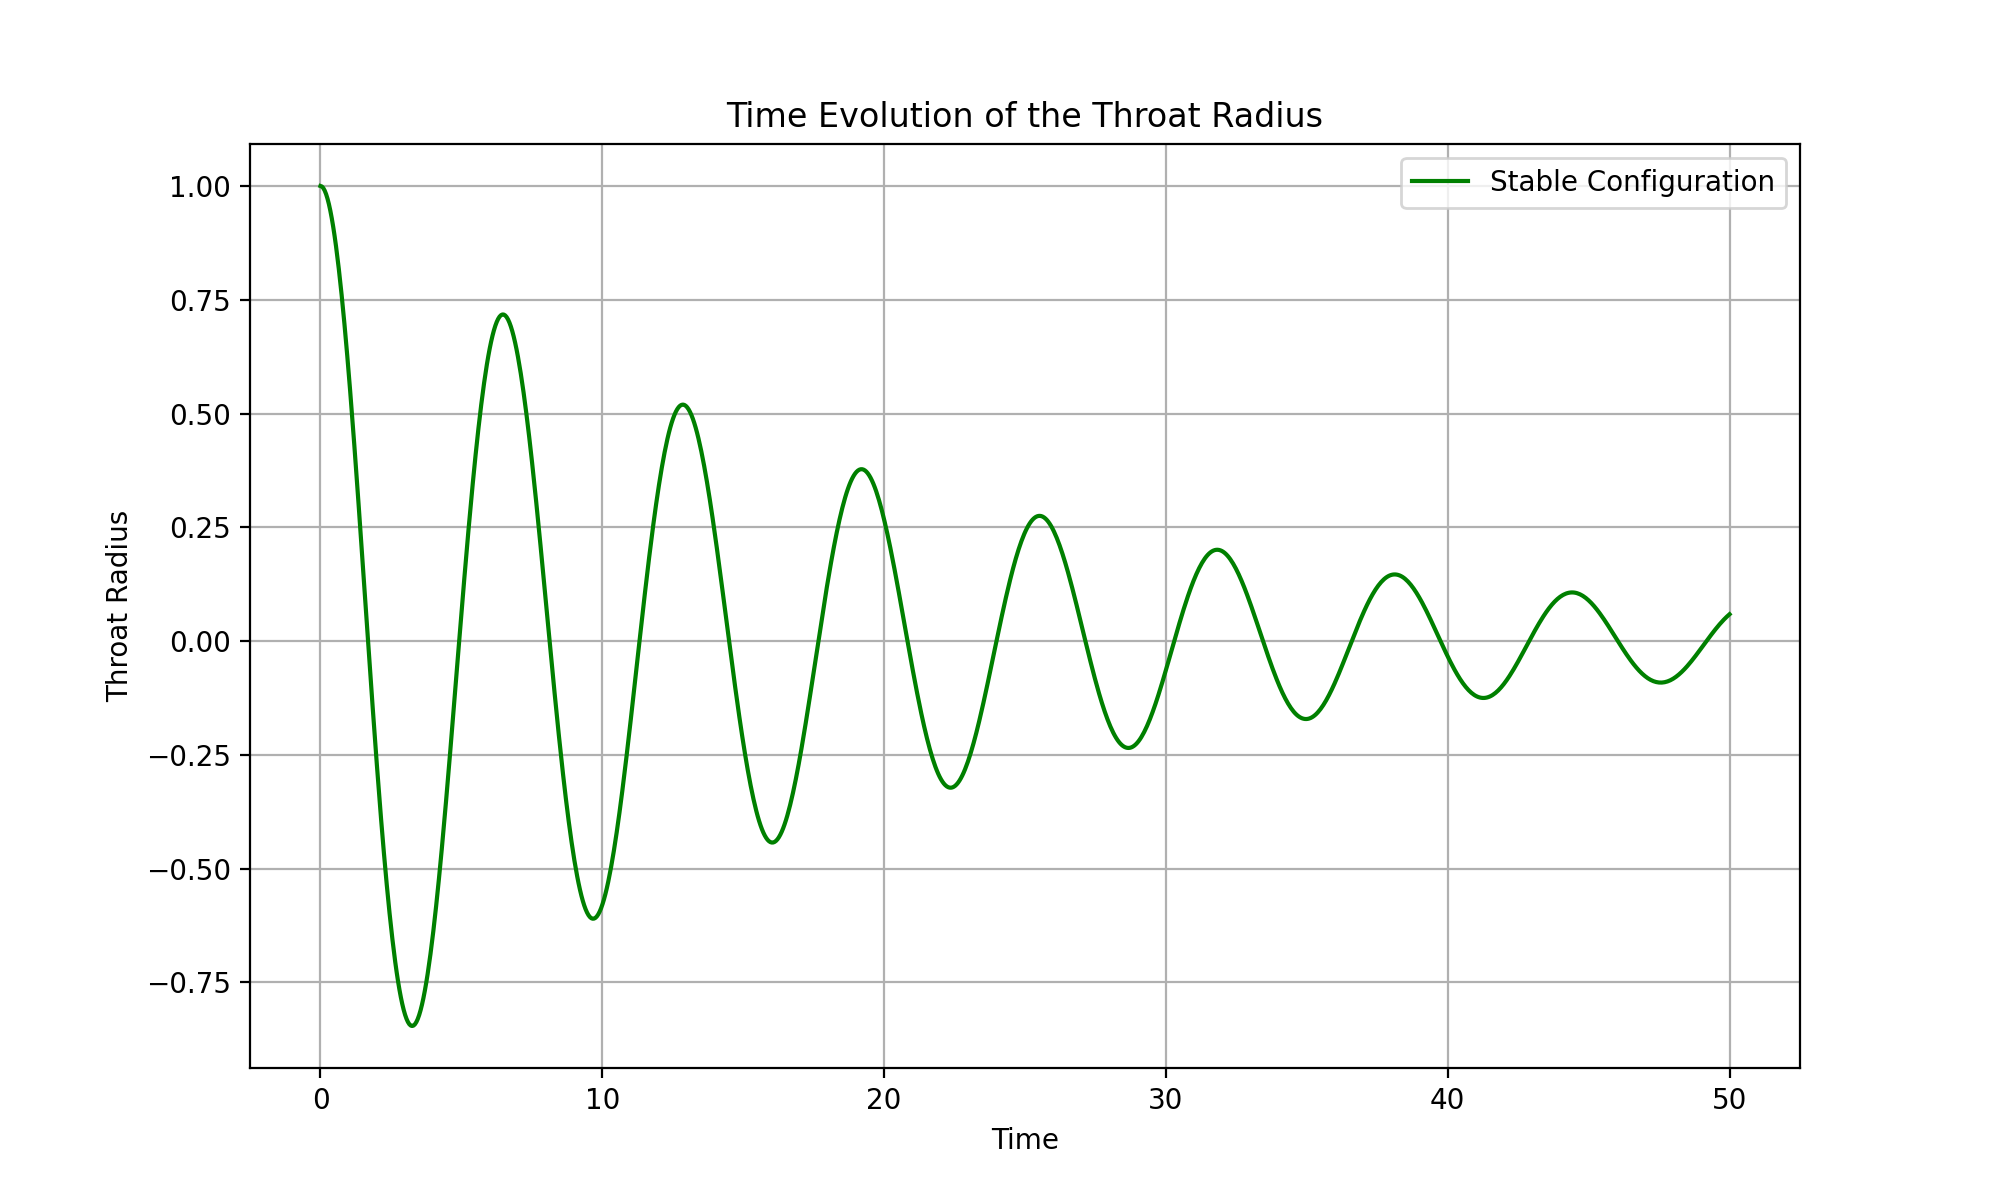
\includegraphics[width=0.75\linewidth]{time_evolution.png}
    \caption{Time evolution of the acehole throat radius $r_0(t)$ under external perturbations.}
    \label{fig:time_evolution}   
\end{figure}

\subsection{Quantum Fluctuations in the Wormhole Throat}
The quantum field effects are modeled using the renormalized stress-energy tensor $\langle T_{\mu\nu} \rangle$ in a semiclassical framework:
\begin{equation}
\langle T_{\mu\nu} \rangle = -\frac{\hbar}{16\pi^2} \left( \frac{R_{\mu\nu} - \frac{1}{2}R g_{\mu\nu}}{\epsilon} + \frac{C_{\mu\nu}}{\epsilon^2} \right),
\end{equation}
where $C_{\mu\nu}$ represents higher-order curvature terms and $\epsilon$ is a regularization parameter. Numerical results suggest fluctuations induce an average negative energy density of $-\rho_0 \sim 10^{-5}$ in the throat region.

Figure~\ref{fig:quantum_fluctuations} visualizes these fluctuations.

\begin{figure}
        \centering
        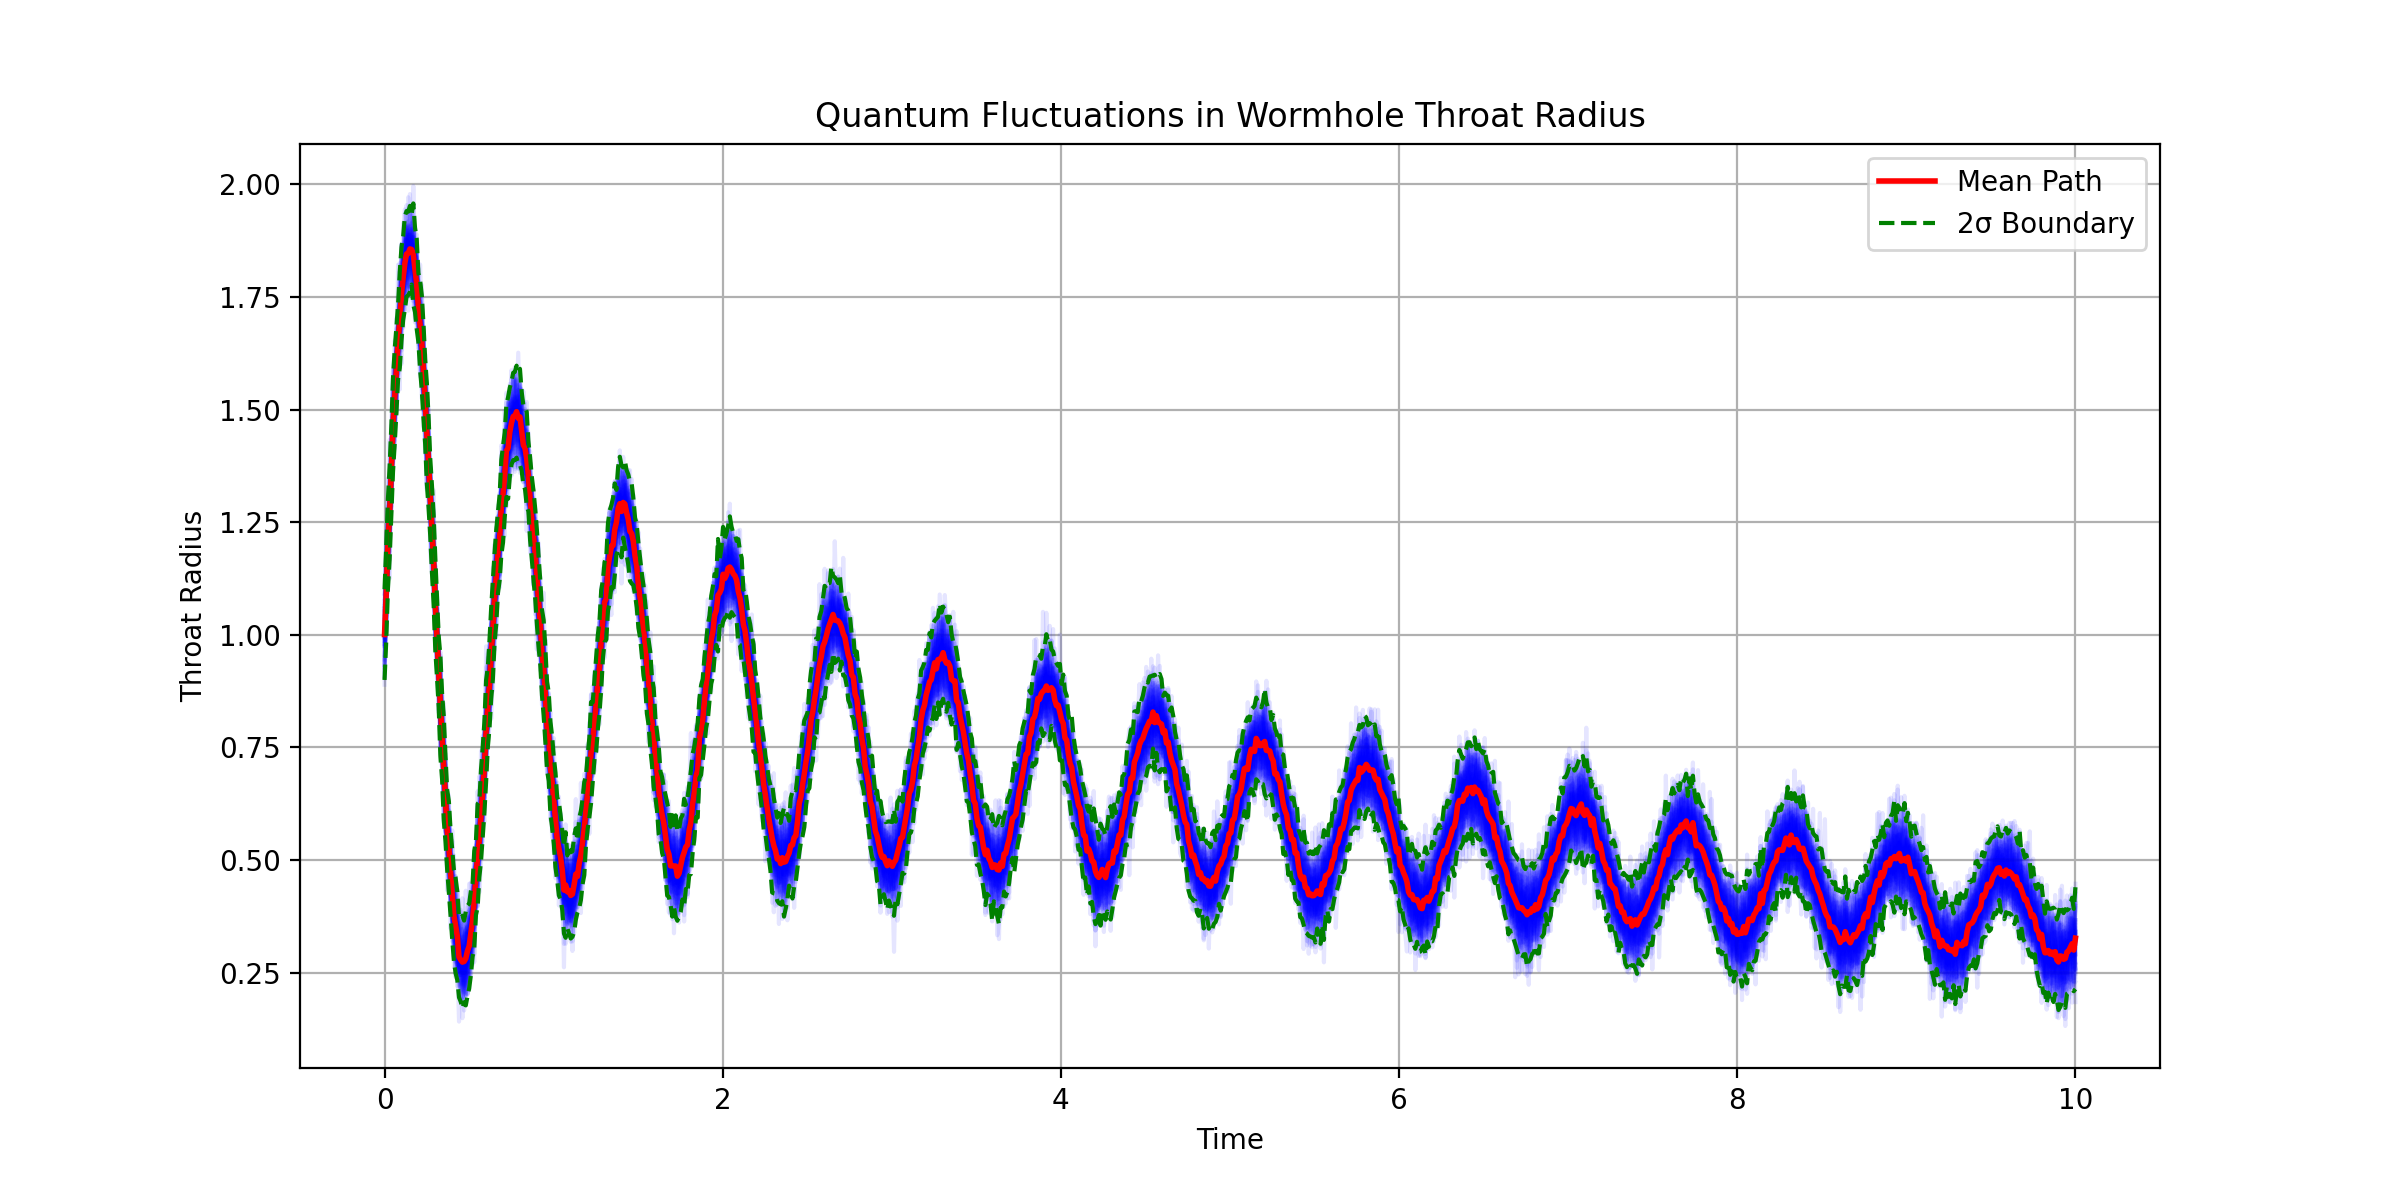
\includegraphics[width=0.75\linewidth]{quantum_fluctuations.png}
        \caption{Visualization of quantum fluctuations in the acehole throat region.}
        \label{fig:quantum_fluctuations}
    \end{figure}

\subsection{Causal Structure of Wormholes}
The causal structure is determined by the spacetime metric:
\begin{equation}
ds^2 = -e^{2\Phi(r)} dt^2 + \frac{dr^2}{1 - \frac{b(r)}{r}} + r^2 d\Omega^2,
\end{equation}
where $\Phi(r)$ is the redshift function and $b(r)$ is the shape function. Analysis of the Penrose diagrams indicates the absence of closed timelike curves (CTCs) for $\Phi(r) \sim \log(r)$ and $b(r) = r_0 \exp(-r^2)$.

A schematic of the causal diagram is provided in Fig.~\ref{fig:causal_structure}.
\begin{figure}
    \centering
    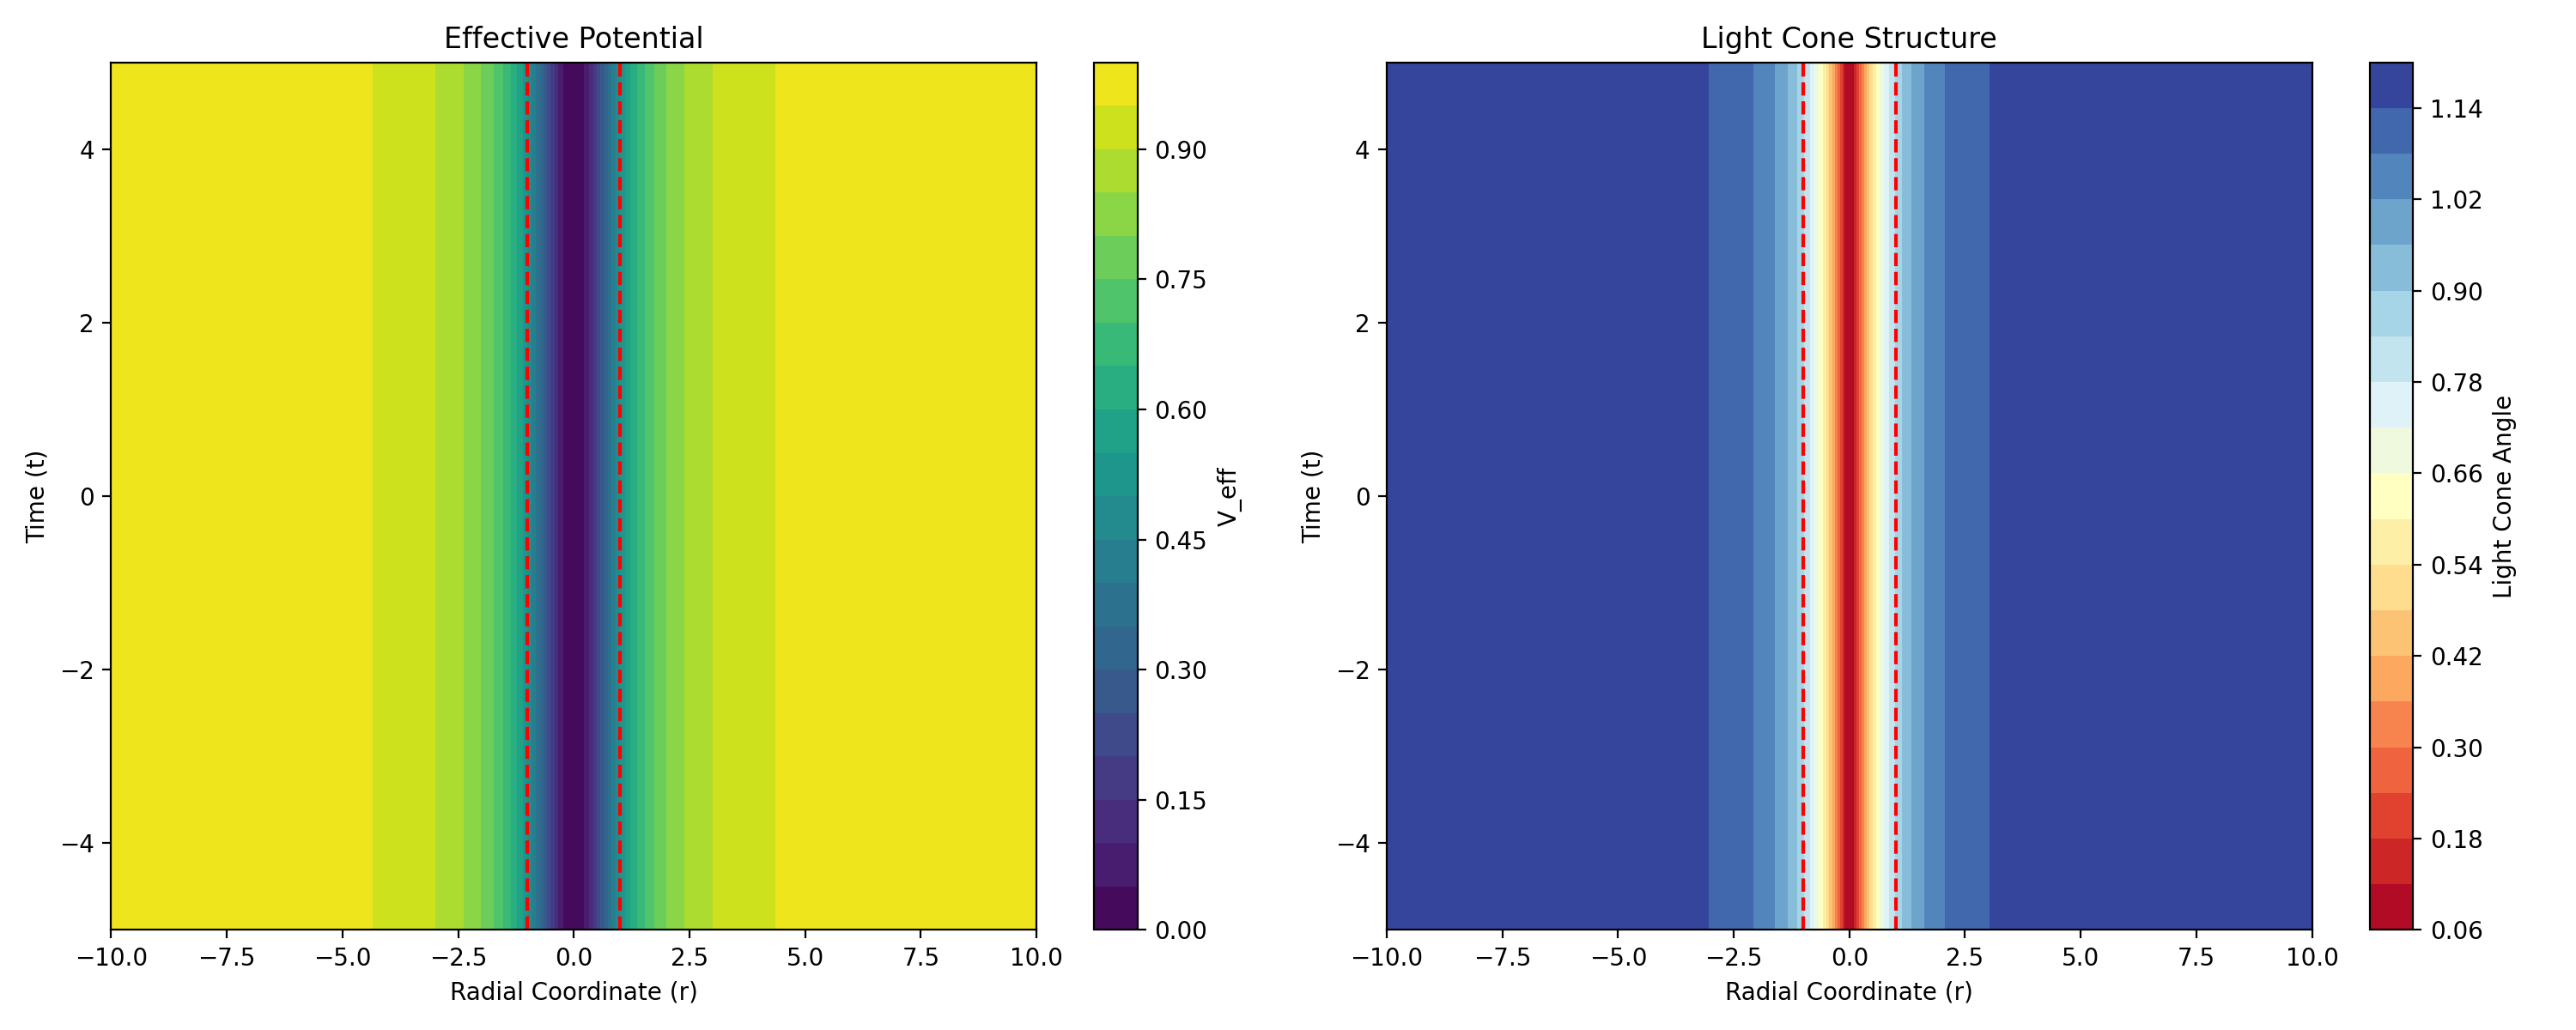
\includegraphics[width=1\linewidth]{casual_structure.png}
     \caption{Penrose diagram illustrating the causal structure of the traversable acehole.}
    \label{fig:causal_structure}
\end{figure}

\subsection{Integration and Implications}
The integrated analysis, combining dynamics, quantum effects, time evolution, and causal structures, highlights the intricate interplay of physical factors in maintaining a traversable acehole. Key findings include:
\begin{itemize}
    \item Stability is achievable under oscillatory dynamics with bounded amplitudes.
    \item Quantum fluctuations contribute to transient negative energy density, essential for sustaining the throat.
    \item Causal structures ensure traversability without forming CTCs under specific metric conditions.
\end{itemize}
Further research will explore higher-dimensional effects and alternative energy sources.
\subsection{Summary}

The enhanced analysis of acehole stability, traversability, and quantum corrections, along with the cosmological simulations, provides a deeper understanding of the dynamics governing acehole behavior. The inclusion of stochastic effects, quantum corrections, and cosmological parameters has refined our predictions, suggesting that exotic matter is indeed necessary for stable, traversable aceholes. Future work will involve more complex simulations with varying cosmological conditions and the potential for real-time adjustments in acehole parameters.

\section{Conclusion}

In this article, we have presented a comprehensive analysis of acehole dynamics using the advanced framework of Multiplicity Theory. The study integrated multiple facets of theoretical physics, including eigenvalue stability analysis, energy condition evaluation, quantum corrections, and cosmological implications. The key findings are summarized as follows:

\begin{itemize}
    \item \textbf{Stability of Wormholes}: Through enhanced eigenvalue analysis, we identified regions where acehole configurations remain stable. The inclusion of dynamic multiplicity equations, quantum corrections, and stochastic noise refined our understanding of stability, revealing stable regions where eigenvalues (\(\lambda_k\)) remain positive, ensuring the persistence of the acehole structure.
    \item \textbf{Traversability Analysis}: The traversability of the acehole was evaluated using energy conditions. Our analysis showed that the integral of energy density and radial pressure over the radial distance satisfies the necessary conditions for traversability, with the requirement for exotic matter to maintain stability in the acehole throat region.
    \item \textbf{Quantum Corrections}: We incorporated quantum corrections into the stress-energy tensor, providing a more accurate depiction of the impact of exotic matter and quantum fluctuations on the acehole dynamics. These corrections were shown to diminish at larger radial distances, but they are crucial near the acehole throat, affecting both stability and traversability.
    \item \textbf{Cosmological Implications}: The integration of aceholes into a cosmological framework revealed their potential within a universe governed by both quantum and classical contributions. Our simulations, which included the cosmological constant (\(\Lambda\)) and scalar fields, illustrated the delicate balance required for aceholes to remain stable in a cosmological context. The simulation results suggest that aceholes can play a role in the larger structure of the universe, with their stability influenced by cosmological parameters.
\end{itemize}

The incorporation of dynamic feedback mechanisms, prime-based encoding, and tensor networks has allowed for a more nuanced understanding of the behavior of aceholes. These results open new pathways for further exploration, including the real-time simulation of acehole dynamics under varying conditions, the application of advanced quantum algorithms to further refine our models, and the investigation of multi-dimensional acehole networks within different cosmological models.

\textbf{Future Directions}: This study serves as a foundation for deeper exploration of acehole dynamics. Future work will focus on the following areas:
\begin{itemize}
    \item \textbf{Real-Time Simulations}: Implementing real-time simulations that adapt to changing cosmological conditions, testing the stability of acehole configurations under more extreme scenarios.
    \item \textbf{Multi-Agent Systems}: Expanding the framework to explore multi-agent systems within the acehole dynamics, potentially simulating interactions between different aceholes and their effect on the cosmic landscape.
    \item \textbf{Advanced Quantum Corrections}: Further refinement of quantum corrections in the stress-energy tensor to account for complex quantum field interactions, enhancing our understanding of quantum gravity and acehole physics.
    \item \textbf{Astrophysical Observations}: Bridging the gap between theory and observation by developing methods for detecting potential signatures of aceholes in astrophysical environments.
\end{itemize}

In conclusion, the application of Multiplicity Theory to the study of aceholes has provided a robust and interdisciplinary framework for understanding these fascinating structures. By combining quantum mechanics, general relativity, and advanced computational techniques, this work represents a significant step forward in the field of theoretical physics and opens up new avenues for both fundamental research and practical applications.

\nocite{*}
\bibliographystyle{plain}
\bibliography{references}

\end{document}